\chapter{Conceito do projeto}
\label{chap:fundteor}
%--------- NEW SECTION ----------------------
\section{Webots}
O software Projeta facilmente simulações robóticas completas usando a biblioteca de ativos Webots que inclui
robôs, sensores, atuadores, objetos e materiais.
\subsection{PIONEER}
Veículo terrestre não tripulado (VTNT) da empresa Adept MobileRobots.
São equipados com sonares e enconders, possibilitando, por exemplo, o mapeamento de um ambiente desconhecido.
\begin{figure} [h!]	
   \centering
   \caption{PIONEER}
   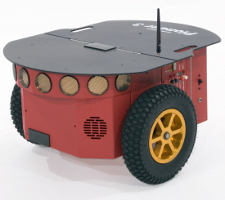
\includegraphics[width=0.4\textwidth]{pioneer.png}
   \caption*{Fonte:robotica.ufv.br/laboratorios/.}
   \label{fig:pioneer}
\end{figure}	


\subsection{Sensor de distância} 
O sensor de distância, é um tipo de sensor que mede a distância entre o robô e um objeto desejado.
Abaixo pode ser visto 16 feiches que representam as posições dos sensores de distância do Pioneer no Webots.

\begin{figure} [h!]	
   \centering
   \caption{Representação do sensor de distância}
   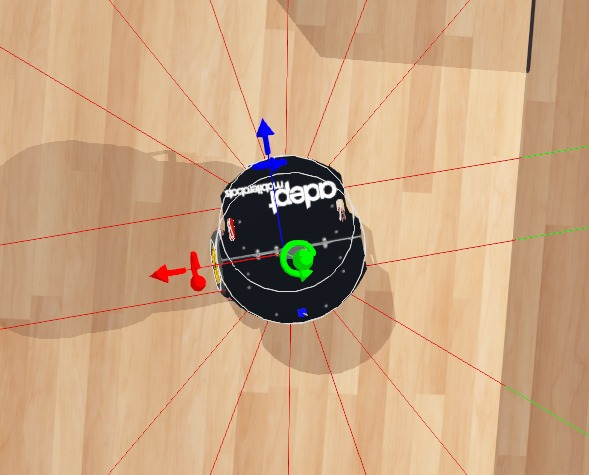
\includegraphics[width=0.4\textwidth]{sensord.png}
   \caption*{Fonte:Própria.}
   \label{fig:sensordistancia}

\end{figure}	

\subsection{Sensor de Luminosidade} 
sensor é medir a intensidade de luz do ambiente ao seu redor, variando o estado de sua saída digital caso detectado um determinado nível de luminosidade. 
Abaixo pode ser visto um cubo amarelo que representa o sensor luminosidade adicionado no Pioneer.

\begin{figure} [h!]	
   \centering
   \caption{Representação do sensor de luminosidade}
   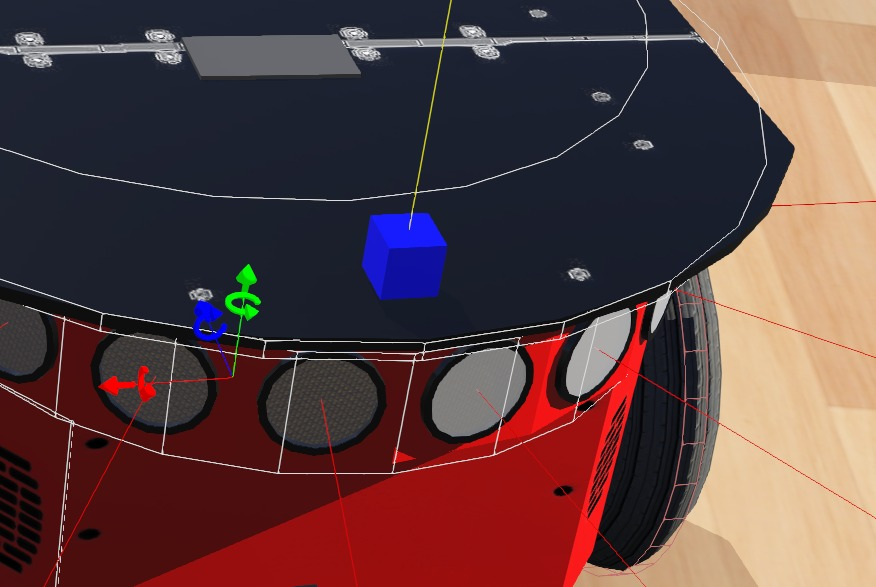
\includegraphics[width=0.4\textwidth]{sensorl.jpeg}
   \caption*{Fonte:Própria.}
   \label{fig:sensorluminosidade}
\end{figure}	

\section{Turtlesim}
\subsection{Nós ROS}
Um nó é apenas um arquivo executável dentro de um pacote do ROS. Nós no ROS usam bibliotecas clientes para se comunicar com outros nós.
Nós podem publicar e/ou subscrever em tópicos, além de poderem prover serviços também.
\subsection{tópicos ROS}
Nós podem publicar menssagens em tópicos assim como podem subescrever menssagens de tópicos.
Como é o exemplo dos nós turtlesim e turtle-teleop-key que se comuniçam entre si através do tópico turtle1command-velocity
turtle-teleop-key está publicando a tecla digitada no tópico, enquanto o turtlesim subescreve o mesmo tópico para receber a tecla digitada. 
A imagem abaixo mostra os nós turtlesim e teleop, e o tópico command-velocity que faz a comunicação entre os dois nós.

\begin{figure} [h!]	
   \centering
   \caption{nós e tópicos ROS}
   
\includegraphics[width=0.6\textwidth]{net1.jpeg}
   \caption*{Fonte:Tutorials-UnderstandingTopics}
   \label{fig:nosetopicos}
\end{figure}	
\subsection{Publisher e Subscribers}
Publisher publica as informações ou mensagens no tópico e o subscriber subscreve o tópico e recebe as informações publicadas.
As mensagens são transmitidas em um tópico e cada tópico possui um nome exclusivo na rede ROS. Se um nó deseja compartilhar informações,
ele usa publisher para enviar dados a um tópico. Um nó que deseja receber essas informações usa subscriber desse mesmo tópico. 
Além de seu nome exclusivo, cada tópico também possui um tipo de mensagem , que determina os tipos de mensagens que podem ser transmitidas naquele tópico.
O conceito de publisher e subscriber pode ser melhor visto na figura abaixo.
\begin{figure} [h!]	
   \centering
   \caption{publisher e subscriber ROS}
   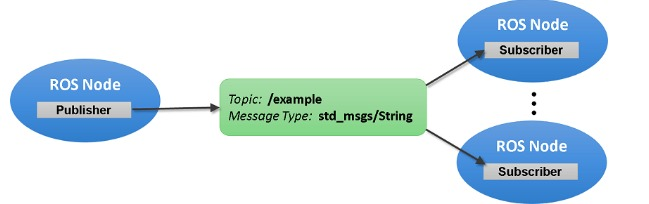
\includegraphics[width=0.6\textwidth]{sep.jpeg}
   \caption*{Fonte:la.mathworks.com/help//ros/ug/exchange-data-with-ros-publishers-and-subscribers.html}
   \label{fig:publisheresubscriber}
\end{figure}	
\subsection{Services e messages}
Os nós comunicam-se entre si publicando mensagens em tópicos . Uma mensagem é uma estrutura de dados simples, composta por campos digitados.
Os nós também podem trocar uma mensagem de solicitação e resposta como parte de uma chamada de serviço ROS .
O modelo publisher e subscriber é um paradigma de comunicação muito flexível, mas seu transporte unilateral para muitos não é apropriado
para interações de solicitação e resposta RPC, que geralmente são necessárias em um sistema distribuído. 
A solicitação e resposta é feita por meio de um Serviço, que é definido por um par de mensagens : uma para a solicitação e outra para a resposta.
\begin{figure} [h!]	
   \centering
   \caption{services e messages ROS}
   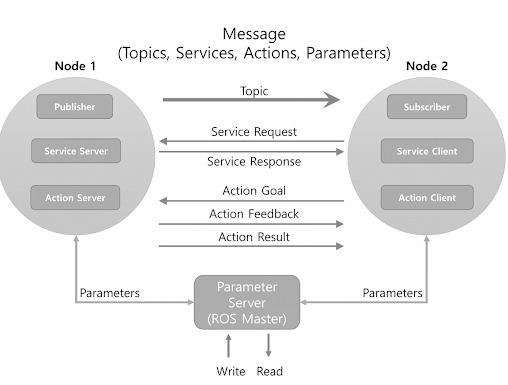
\includegraphics[width=0.6\textwidth]{sem.jpeg}
   \caption*{Fonte:robinrobotic.blogspot.com/2019/06/ros-terminology.html}
   \label{fig:servicesemessages}
\end{figure}	
 \section{Husky}
 %desenvolver mais
 Além disso, o Walker deve realizar um desafio, que consiste em navegar de forma autônoma, se localizar por meio de tags e encontrar um determinado objeto.
 \section{CPP workbook}
 \section{Python workbook1e2}
%----------------------------------------------------------

%--------- NEW SECTION ----------------------


%---------------picture------------------------------------
% \begin{figure}
%     \centering
%     \subfigure[Figure A]{\label{fig:a}\includegraphics[width=60mm]{./lq}}
%     \subfigure[Figure B]{\label{fig:b}\includegraphics[width=60mm]{./lq}}
%     \subfigure[Figure C]{\label{fig:c}\includegraphics[width=\textwidth]{./lq}}
%     \caption{Three simple graphs}
%     \label{fig:three graphs}
% \end{figure}
%----------------------------------------------------------

% \begin{figure}
%     \centering
%     \begin{subfigure}[b]{0.3\textwidth}
%         \centering
%         \includegraphics[width=\textwidth]{./lq}
%         \caption{$y=x$}
%         \label{fig:y equals x}
%     \end{subfigure}
%     \hfill
%     \begin{subfigure}[b]{0.3\textwidth}
%         \centering
%         \includegraphics[width=\textwidth]{./lq}
%         \caption{$y=3sinx$}
%         \label{fig:three sin x}
%     \end{subfigure}
%     \hfill
%     \begin{subfigure}[b]{0.3\textwidth}
%         \centering
%         \includegraphics[width=\textwidth]{./lq}
%         \caption{$y=5/x$}
%         \label{fig:five over x}
%     \end{subfigure}
%        \caption{Three simple graphs}
%        \label{fig:three graphs}
% \end{figure}


% %--------- NEW SECTION ----------------------
% \section{Assunto 2}
% \label{sec:ass2}
% flkjasdlkfjasdlkfjs

% \begin{table}[h]
%     \begin{subtable}[h]{0.45\textwidth}
%         \centering
%         \begin{tabular}{l | l | l}
%         Day & Max Temp & Min Temp \\
%         \hline \hline
%         Mon & 20 & 13\\
%         Tue & 22 & 14\\
%         Wed & 23 & 12\\
%         Thurs & 25 & 13\\
%         Fri & 18 & 7\\
%         Sat & 15 & 13\\
%         Sun & 20 & 13
%        \end{tabular}
%        \caption{First Week}
%        \label{tab:week1}
%     \end{subtable}
%     \hfill
%     \begin{subtable}[h]{0.45\textwidth}
%         \centering
%         \begin{tabular}{l | l | l}
%         Day & Max Temp & Min Temp \\
%         \hline \hline
%         Mon & 17 & 11\\
%         Tue & 16 & 10\\
%         Wed & 14 & 8\\
%         Thurs & 12 & 5\\
%         Fri & 15 & 7\\
%         Sat & 16 & 12\\
%         Sun & 15 & 9
%         \end{tabular}
%         \caption{Second Week}
%         \label{tab:week2}
%      \end{subtable}
%      \caption{Max and min temps recorded in the first two weeks of July}
%      \label{tab:temps}
% \end{table}